\documentclass[11pt]{article}
\usepackage{geometry}                
\geometry{letterpaper}                   

\usepackage{graphicx}
\usepackage{amssymb}
\usepackage{epstopdf}
\usepackage{natbib}
\usepackage{amssymb, amsmath}
\usepackage{wrapfig}
\usepackage{empheq}

\begin{document}



\section{Simulation results and discussion}
\subsection{Results of the SIR model}
All the values for the compartments s, x and r calculated by the model are within the possible intervals. The best fit values for $\beta_{x}$, $\gamma$ and $\kappa$ are 3.9114, 3.8816 and 7.5279e-12, respectively. The basic reproductive number $R_{0} = \frac{\lambda S}{\gamma}$ is always smaller than 1 because the product of $\lambda S$ is always smaller than $\gamma$. This would predict a non spreading disease or a very mild epidemic (CITE). Figures \ref{fig:mean_susceptible} and \ref{fig:mean_removed} show the mean over all districts for the susceptible and removed compartments, respectively. One can see that the slope of the curve is steadier for the calculated model compared to the observed data. The observed curve of the infectious compartment in figure \ref{fig:mean_infectious} is highly nonlinear and the magnitude is slightly earlier than our calculated data. It is important not only to look at the means but the distribution of s, x and r within Haiti.\\

\begin{figure}[htb]
  %\centering
  \begin{minipage}[t]{0.49\textwidth}
    \centering
    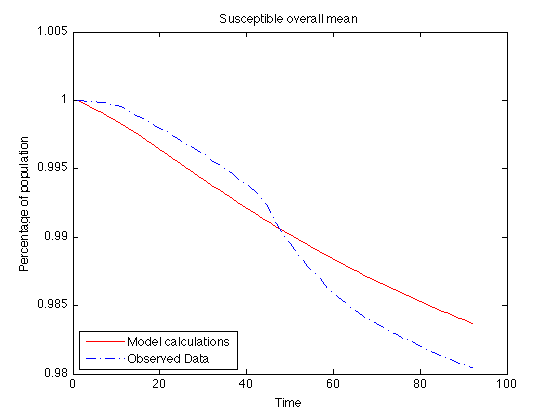
\includegraphics[width=\textwidth]{Bilder/susceptible_mean.png} 
    \caption{Mean over all districts for the susceptible compartment}
	\label{fig:mean_susceptible}
  \end{minipage}
  \hspace{0.02\textwidth}
  \begin{minipage}[t]{0.49\textwidth}
    \centering
    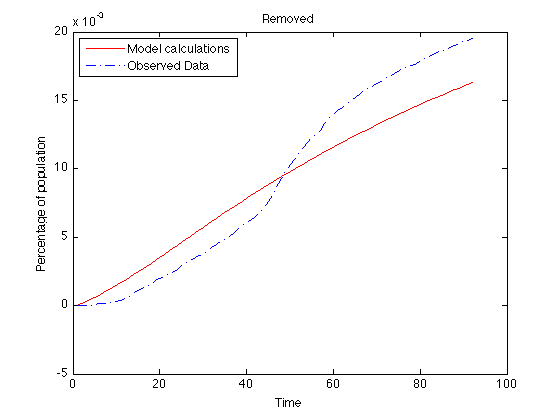
\includegraphics[width=\textwidth]{Bilder/removed_mean.png} 
    \caption{Mean over all districts for the removed compartment}
	\label{fig:mean_removed}
  \end{minipage}
\end{figure}


The plots \ref{fig:all_susceptible}, \ref{fig:all_removed} and \ref{fig:all_infectious} show the observed and calculated values of all ten compartments. The districts Nord, Nord-Est and Grand Anse show an incredible increase and decrease in the removed and susceptible compartments, respectively. These compartments also have unlikely observed data for the infectious compartment, as seen in figure \ref{fig:all_infectious}. In the district Grand Anse the amount of infected people decreases from  0.1\% to 0.04\% within around 3 days. On the other hand, there are some extremely good fits, for instance in the departments Nord-Ouest and Centre. 


\begin{figure}[htb]
  %\centering
  \begin{minipage}[t]{0.49\textwidth}
    \centering
    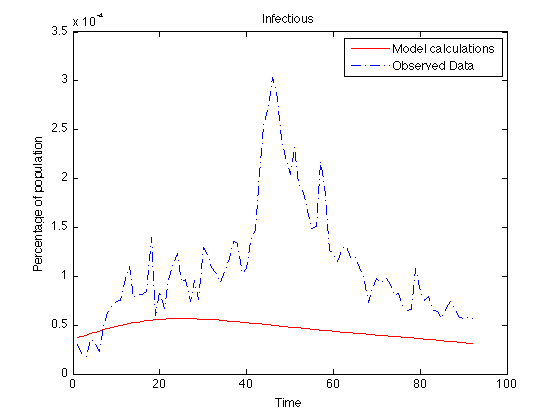
\includegraphics[width=\textwidth]{Bilder/infectious_mean.png} 
    \caption{Mean over all districts for the infectious compartment}
	\label{fig:mean_infectious}
  \end{minipage}
  \hspace{0.02\textwidth}
  \begin{minipage}[t]{0.49\textwidth}
    \centering
    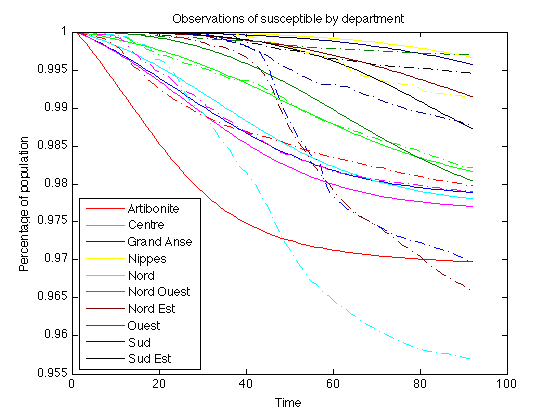
\includegraphics[width=\textwidth]{Bilder/susceptible.png} 
    \caption{Observed and calculated data for all districts of the susceptible compartment}
	\label{fig:all_susceptible}
  \end{minipage}
  
  \hspace{0.15\textwidth}

  %\centering
  \begin{minipage}[t]{0.49\textwidth}
    \centering
    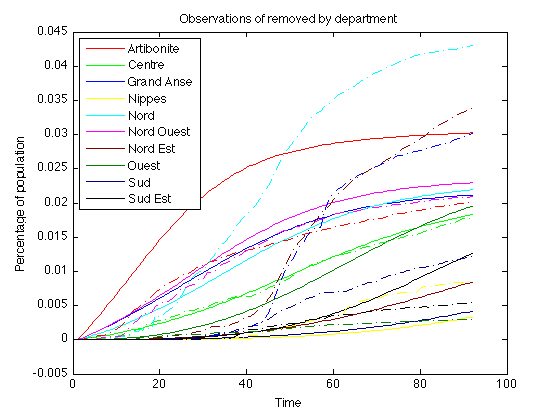
\includegraphics[width=\textwidth]{Bilder/removed.png} 
    \caption{Observed and calculated data for all districts of the removed compartment}
	\label{fig:all_removed}
  \end{minipage}
  \hspace{0.02\textwidth}
  \begin{minipage}[t]{0.49\textwidth}
    \centering
    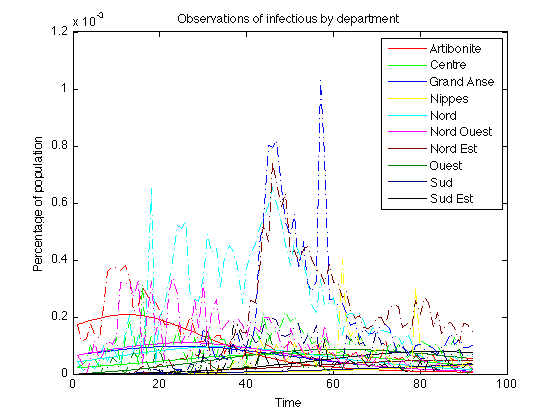
\includegraphics[width=\textwidth]{Bilder/infectious.png} 
    \caption{Observed and calculated data for all districts of the infectious compartment}
	\label{fig:all_infectious}
  \end{minipage}
\end{figure}

One of the benefits of our simple model is the possibility to compare the effect of transmission within the same district versus transmission between districts. The force of infection $\lambda$ consists of two parts, as seen in equation (lambda). Here $\beta_{x}x$ represents the transmission within the same district and $\sum\limits_{j=0}^I  \Theta_{ij}  x_{j$ the transmission between compartments. Figure XX shows the interdepartmental transmission coefficients over time. The best fit of $\beta_{x}=3.9114$ is always around $10^4$ times bigger. This predicts that in our model the transmission within the same district is much more important than the interdepartmental transmission.


\begin{figure}[h]
  %\centering
  \begin{minipage}[t]{\textwidth}
    \centering
    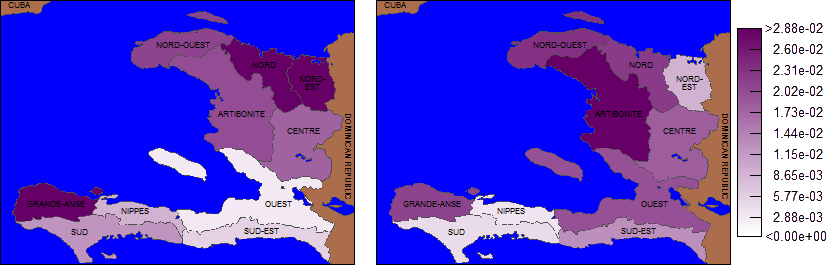
\includegraphics[width=\textwidth]{Bilder/geo_removed.png} 
    \caption{Geographical display of observed and calculated removed data at t=92}
	\label{fig:geo_removed}
  \end{minipage}
\end{figure}

Figure \ref{fig:geo_removed} shows the spread of the removed compartment on the 1st of January 2011. Here the observed data is shown on the left while our calculated data is on the right. Our model predicts the spatial spread of the disease to some extent quite well. After the change of initial conditions in the infectious compartment for the district Grand Anse we were able to also predict the spread in the far west. Our calculated least-infected districts are Sud and Nippes. The observed data show that they are further to the east, namely Ouest and Sud-Est. Our model also calculates the highest-infected district to be Artibonite, whereas the observed data shows that they are Nord-Est and Nord.



\subsection{Discussion} 
The reliability and accessibility of data have proved to be a crucial part of building this model. Because of the lack of water quality data we have decided to construct an ordinary SIR model instead of an SIWR. Even with our simplified SIR model equations we were able to predict the epidemic over 3 months to some extent. In our model, the interdepartmental transmission is of no importance to the spread of the disease. There are two main reasons we believe why this might be in our model. Tien and Earn (CITE) put the percentage of infected, susceptible and infectious populations in relation to the area observed in the model. For us this would mean we put the respective percentages in relation to the area of the districts. The result would be a density, for instance percent infected per square kilometer. For districts with many inhabitants in a relatively small area this would result in much higher values for s,x and r compared to sparsely inhabited districts. When using the gravity model as proposed by Tuite et al. (CITE) the districts with a high x would have a much greater influence on the force of infection $\lambda$.\\
Another reason might be the gravity model we used in itself. Because we chose a different way of rescaling our values, s,x and r are much higher than those calculated by Tuite et al. (CITE). As a result the relation $\frac{pop_{i}*pop_{j}}{d^{n}}$ might be unsuited for our dimensions. We tried to even this out by fitting $\kappa$.









\end{document}